\section{Durchführung}
\label{sec:Durchführung}

\subsection{Aufbau}

In Abbildung \ref{fig:VA} ist der Versuchsaufbau skizziert.
Durch Strahlungseinfall wird im Zählrohr die Ladung $Q$ am Draht gesammelt.
Am Widerstand $R$ wird daraus ein Spannungsimpuls erzeugt, der dann am
Kondensator $C$ ausgekoppelt wird. Das erzeugte Signal kann über einen
Verstärker mit dem Zähler oder auch am Oszillographen detektiert werden.

\begin{figure}
  \centering
  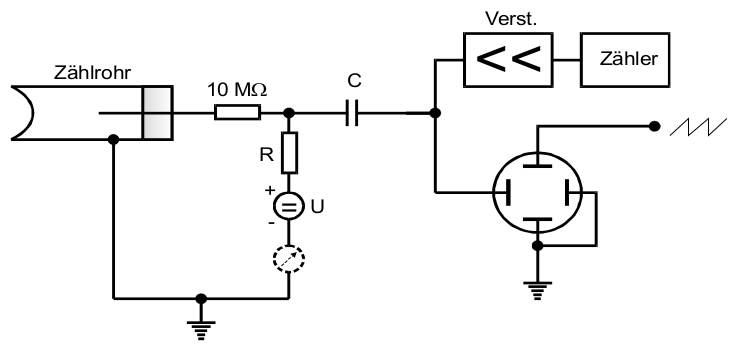
\includegraphics[height=5cm]{MeinePics;)/VA.png}
  \caption{Skizze des Versuchsaufbaus.\cite{anleitung}}
  \label{fig:VA}
\end{figure}

Für den gesamten Versuch wird der $\beta$-Strahler \ce{^{204}_{81}Tl} verwendet.

\subsection{Messprogramm}

Bei den Teilversuchen sollte die Betriebsspannung des Zählrohrs
$\SI{720}{\volt}$ nicht überschreiten, da sonst Schäden entstehen könnten.

\subsubsection{Zählrohrcharakteristik und Ladung pro Teilchenimpuls}
\begin{enumerate}
  \item Zunächst wird am Zähler eine Impulsrate von $\SI{10}{\per\second}$ eingestellt
  und der gegebene $\beta$-Strahler vor das Zählrohr eingespannt.
  \item Es werden für insgesamt 26 verschiedene Spannungen Stromstärke und
  Impulse notiert, um Zählrohrcharakteristik und Ladung zu bestimmen.
\end{enumerate}

\subsubsection{Nachentladung}
\begin{enumerate}
  \item Bei $\SI{350}{\volt}$ und $\SI{700}{\volt}$ wird jeweils der Abstand
  zwischen Primär- und Nachentladungsimpuls gemessen.
\end{enumerate}

\subsubsection{Messung der Totzeit}
\begin{enumerate}
  \item Es wird eine Betriebsspannung von $U = \SI{600}{\volt}$ und
  eine Impulsrate von $\SI{60}{\per\second}$ am Zähler eingestellt.
  \item Zunächst werden Totzeit und Erholungszeit des Zählrohrs am Oszilloskop
  gemessen und notiert.
  \item Mit der Zwei-Quellen-Methode wird die Totzeit des Zählrohrs ein weiteres
  mal bestimmt.
\end{enumerate}
